\documentclass[a4paper, 12pt]{article}

\usepackage[english, russian]{babel}
\usepackage[T2A]{fontenc}
\usepackage[utf8]{inputenc}
\usepackage{mathtext}
\usepackage{amsfonts}
\usepackage{ amssymb }
\usepackage{amsmath}
\usepackage{graphics}
\usepackage{graphicx}
\usepackage{wrapfig}
\usepackage{geometry}
\usepackage{float}
\geometry{
	a4paper,
	total={170mm, 257mm},
	left=20mm,
	top=10mm}

\title{Лабораторная работа 3.4.2. Закон Кюри-Вейсса}
\author{Абакшин Василий, Б05-207}
\date{\today}

\begin{document}
	\maketitle
	
	\section*{Краткая теория}
	В данной лабораторной работе предлагается проверить закон Кюри-Вейсса: при температуре выше температуры Кюри:
	\[\chi \sim \frac{1}{T - \theta_P}\]
	$\theta_P$ - парамагнитная точка Кюри.\\
	Исследуемый материал будет помещен в катушку индуктивности, из-за чего её индуктивность будет меняться с температурой:
	\[L - L_0 \sim \mu - 1 = \chi\]
	Изменение индуктивности будем наблюдать с помощью изменения периода колебаний: $\tau = 2\pi\sqrt{LC}$, поэтому 
	\[L - L_0 \sim \tau^2 - \tau_0^2 \ \rightarrow \ \chi \sim \tau^2 - \tau_0^2 \ \ \rightarrow \ \frac{1}{\tau^2 - \tau_0^2} \sim T - \theta_P\]
	Здесь $L_0$ и $\tau_0$ - индуктивность и период колебаний без образца в катушке соответственно.
	\section*{Экспериментальная установка}
	
	Исследуемый ферромагнитный образец (гадолиний) расположен внутри пустотелой катушки самоиндукции, которая служит индуктивностью колебательного контура, входящего в состав $L C$ -автогенератора.
	
	\begin{center}
		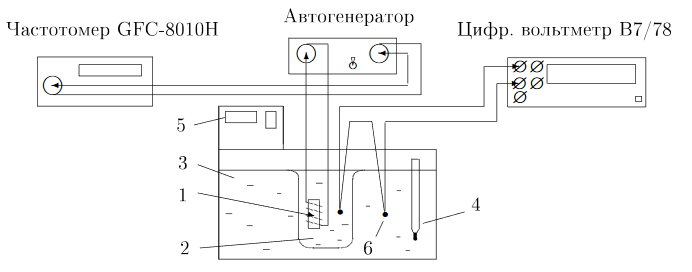
\includegraphics[width=0.8\textwidth]{1.png}
		\label{pic1}
	\end{center}
	Катушка 1 с образцом помещена в стеклянный сосуд 2, залитый трансформаторным маслом. Масло предохраняет образец от окисления и способствует ухудшению электрического контакта между отдельными частичками образца. Кроме того, оно улучшает тепловой контакт между образцом и рабочей жидкостью 3 в термостате. Ртутный термометр 4 используется для приближённой оценки температуры.\\
	При изменении температуры меняется магнитная восприимчивость образца $\chi,$ а следовательно, самоиндукция катушки и период колебаний $\tau$ автогенератора. Для измерения периода используется частотомер. \\
	Измерения проводятся в интервале температур от $14^{\circ} \mathrm{C}$ до $40^{\circ} \mathrm{C} .$ 
	Температура исследуемого образца всегда несколько отличается от температуры дистиллированной воды в сосуде. Эта разность температур фиксируется термопарой, чувствительность которой $\mathrm{K}=24\frac{\text{град}}{\text{мВ}}$. ЭДС термопары измеряется цифровым вольтметром.
	
	
	\section* {Результаты измерений и их обработка}
	Полученные значения $\tau$ при разных температурах записаны в таблице. Показания цифрового вольтметра изменялись достаточно сильно, поэтому примем их погрешность $\sigma_U = 0,002$ мВ, что в измерении температуры даст погрешность $0,05^{\circ} C$. Вместе с погрешностью измерения температуры в термостате $0,05^{\circ}$ получаем погрешность $0,07^{\circ} C$ в измерении температуры образца.\\
	Период колебаний без образца внутри катушки: $\tau_0 = 6,9092$ мкс.
	\begin{table}[h!]
		\centering
		\begin{tabular}{|c|c|c|c|}
			\hline
			$t, ^{\circ}C$ & $\Delta U$, мВ & $t_{\text{обр}}, ^{\circ} C$ & $\tau$, мкс \\ \hline
			14,15 & -0,0100 & 13,91 & 7,923 \\ \hline
			16,08 & -0,013 & 15,768 & 7,865 \\ \hline
			18,14 & -0,0045 & 18,032 & 7,738 \\ \hline
			20,10 & -0,009 & 19,884 & 7,583 \\ \hline
			22,10 & -0,007 & 21,932 & 7,366 \\ \hline
			24,10 & -0,006 & 23,956 & 7,197 \\ \hline
			28,10 & -0,016 & 27,716 & 7,091 \\ \hline
			32,07 & -0,0165 & 31,674 & 7,044 \\ \hline
			36,09 & -0,007 & 35,922 & 7,016 \\ \hline
			40,07 & -0,014 & 39,734 & 7,003 \\ \hline
		\end{tabular}
		\caption{Значения периода колебаний в зависимости от температуры образца}
	\end{table}
	
	По этим данным строит график $\frac{1}{\tau^2 - \tau_0^2} = f(T)$. Аппроксимируем прямой часть графика, начиная с пятого значения. Получили прямую $y \approx 0,035x - 0,58$. Тогда она пересечет ось абсцисс в точке $\theta_P = (16,84 \pm 1,44) ^{\circ}C \ (\varepsilon = 8,5\%)$
	Точку Кюри по графику определить достаточно сложно, если аппроксимировать первые несколько значений прямой, то точка Кюри будет примерно $\theta = 5,35^{\circ}C$.
	\begin{figure}[h!]
		\centering
		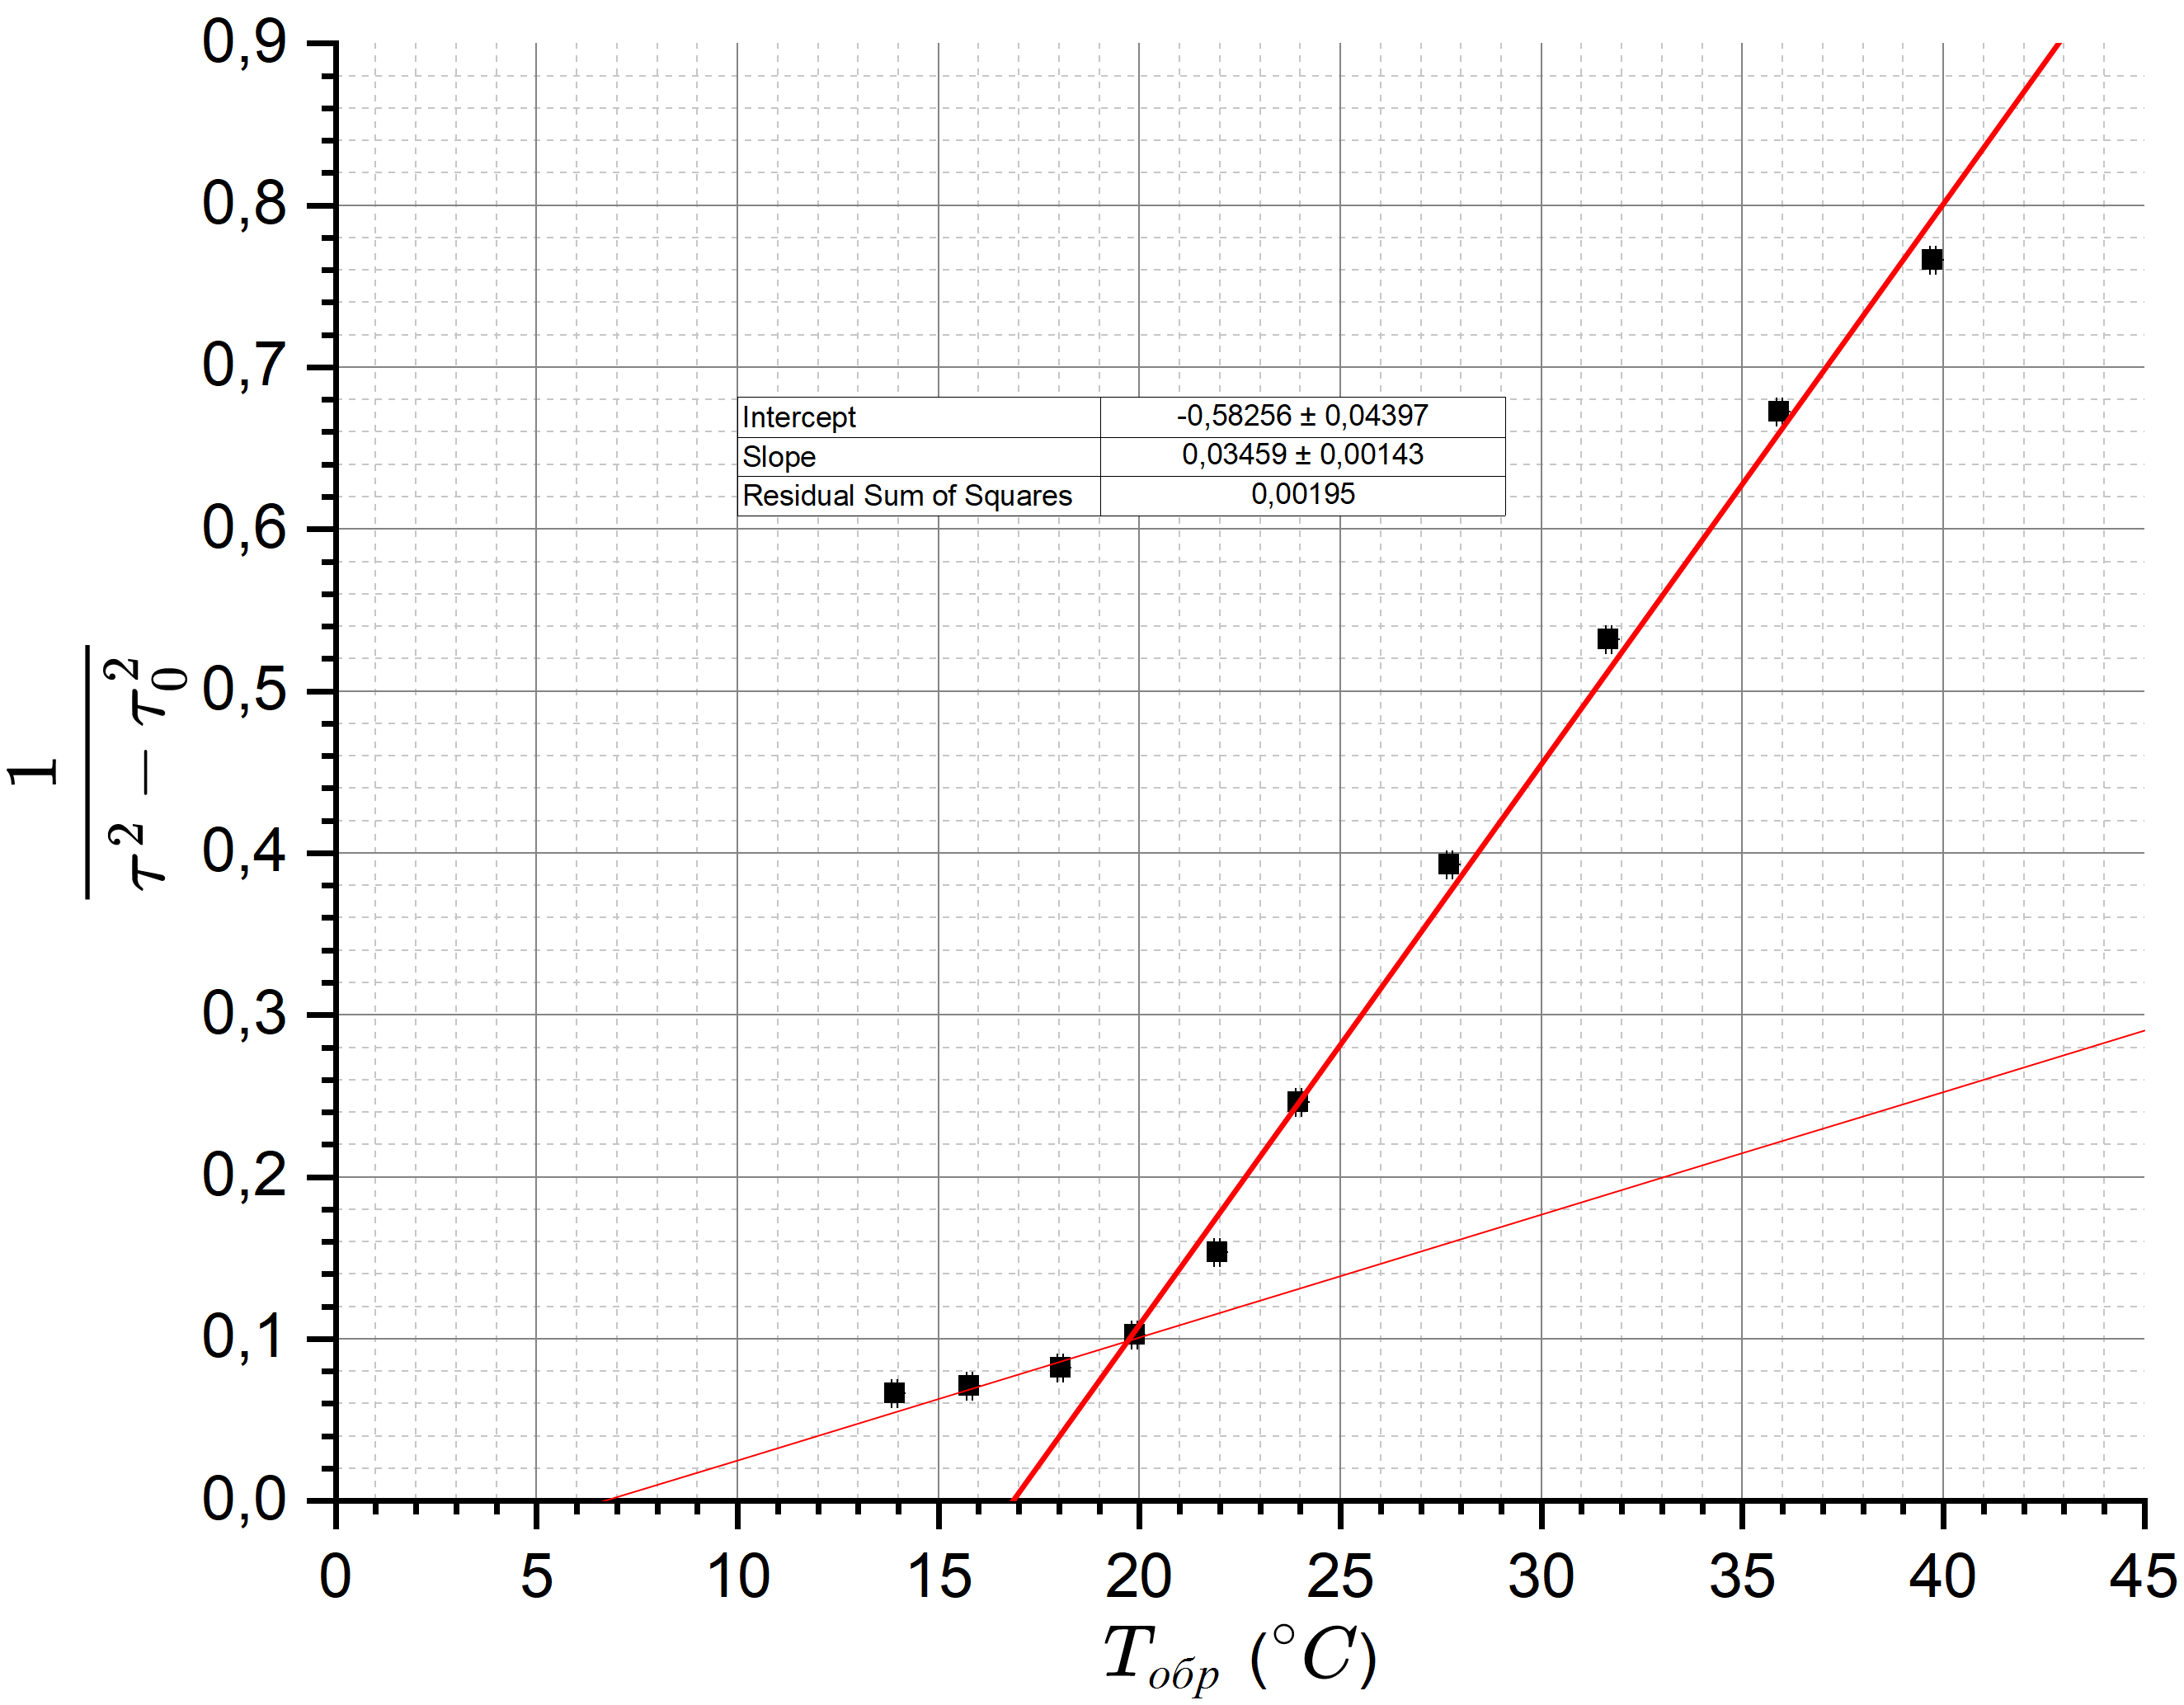
\includegraphics[width = \textwidth]{Veys}
		\caption{Зависимость $\frac{1}{\tau^2 - \tau_0^2} = f(T)$}
	\end{figure}
	\section*{Выводы} 
	В данной лабораторной работе мы проверили выполнимость закона Кюри-Вейсса, получив график зависимости $\frac{1}{\tau^2 - \tau_0^2} = f(T)$. Зависимость совпадает с теоретической по характеру, но значения точки Кюри и парамагнитной температуры Кюри достаточно сильно отличаются от теоретических: $\theta_{th} = 20,2^{\circ}C, \ \ \theta_{P_{th}} > \theta_{th}$. Различия связаны, прежде всего, с способом получения данных: график построен в координатах $\frac{1}{\tau^2 - \tau_0^2} = f(T)$, а $\frac{1}{\tau^2 - \tau_0^2} \sim \frac{1}{\chi}$, то есть строго равенства нет, есть только пропорциональность, а парамагнитная температура Кюри определяется из графика $\frac{1}{\chi}(T)$. Температура Кюри определялась экстраполяцией прямой на нелинейной зависимости, для которой мало точек, поэтому значения неточные.
\end{document}